\section{Air quality visualisations}
The problem of making air quality visible to the general population has been addressed before, from map-based representations to wearable devices and in-city displays. These approaches contemplate new or known ways to tackle the problem of air quality.

\subsection{Table based}
The most basic representation of air quality data is as tabular data, generally including some colours to indicate the quality level of the measurement, as shown in Figure \ref{fig:table_based_visualization}. From these kinds of representations it is easy to read information from multiple places. However, one drawback is that there is too much for the reader to process easily, which is not always pertinent to the reader's current location or requirements. Another issue is that the user requires a previous understanding of the terms and measurements used to annotate the table like \quotes{hourly mean} or \quotes{running 8 hour mean}. 

\begin{figure}[H]
\begin{adjustbox}{width=1\textwidth,center=\textwidth}
  \centering
  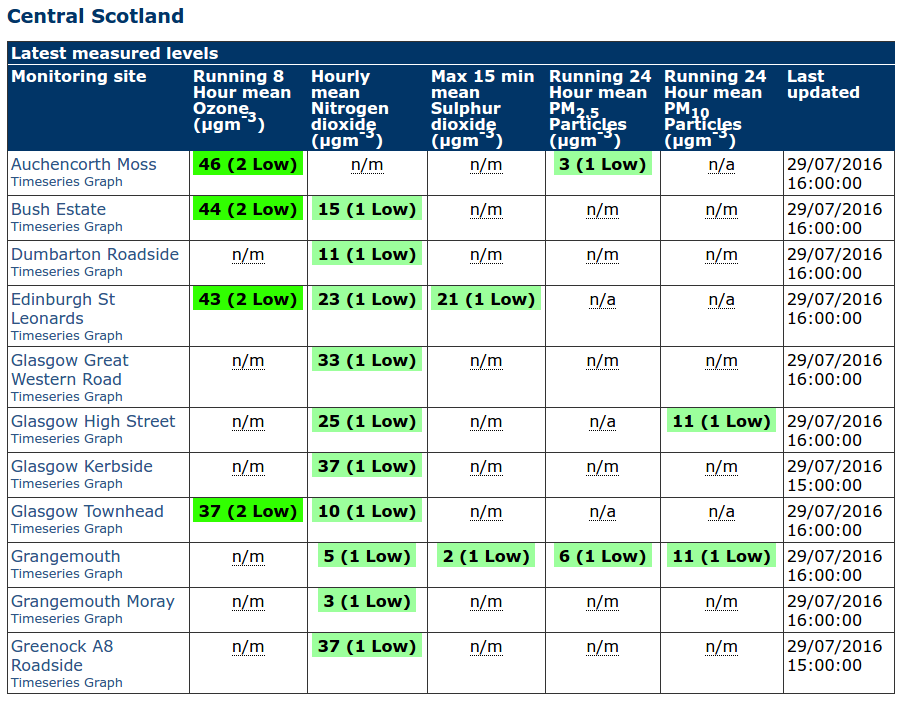
\includegraphics[scale=1]{images/tabular_data.png}
\end{adjustbox}
  \caption[Tabular visualisation]{Tabular visualisation \cite{DepartmentforEnvironment}}
  \label{fig:table_based_visualization}
\end{figure}

\subsection{Map based}
Through maps people can understand where measurements are being made. They are also good for discovering pollution-safe routes when walking around the city or to find out which spots are well suited to physical activity.  Some representations include colour indicators to indicate good or bad levels and allow to read past data by selecting previous dates. However, it is unlikely that one is interested in the measurements for all Scotland's regions, and it is hard to visualise correctly overlaid numeric data on small screens.

\begin{figure}[H]
\begin{adjustbox}{width=1\textwidth,center=\textwidth}
  \centering
  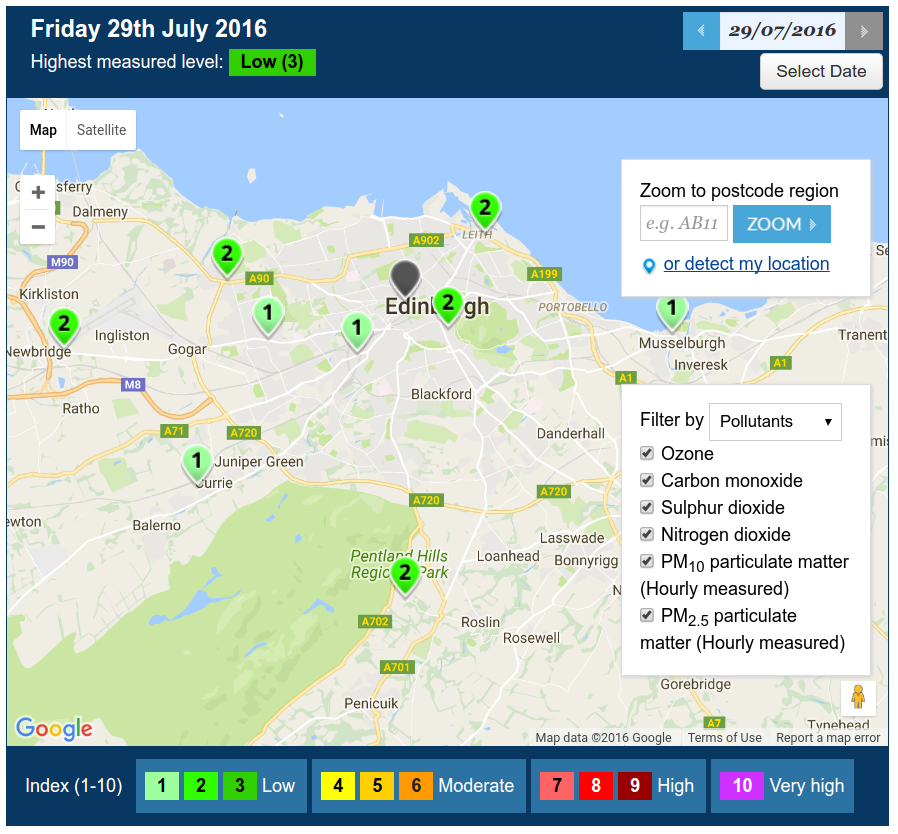
\includegraphics[scale=.30]{images/map_visualization.png}
\end{adjustbox}
  \caption[Map-based visualisation]{Map-based visualisation \cite{Scottishairquality.co.uk2016}}
  \label{fig:web_based_desktop_visualization}
\end{figure}


\subsection{Line based}
Line graphs serve to represent variations of data in defined periods of time, allowing for patterns to be depicted and predictions within the data to be made quickly. It is also possible to include various datasets in one single graph, enabling comparison between them. The inAir project \cite{Kim2013} utilises a line graph to represent indoor particle matter over time. Their findings suggested that this approach allows users to reflect on their behaviours and air quality status, persuading them to modify their practices and decrease their exposure to air pollution. 

\begin{figure}[H]
\begin{adjustbox}{width=1\textwidth,center=\textwidth}
  \centering
  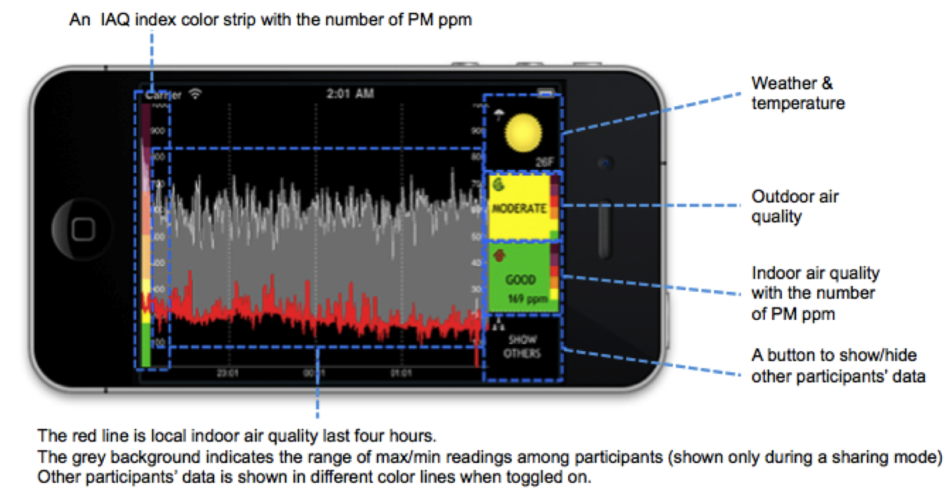
\includegraphics[scale=1]{images/InAir.png}
\end{adjustbox}
  \caption[inAir project: line-based visualisations]{inAir: line-based visualisation\cite{Kim2013}.}
  \label{fig:line_based_inAir}
\end{figure}


\subsection{Photo based}
Photo-based representations as proposed by Lin \cite{Lin2014} allow people to understand levels of pollution by taking pictures of the current environment. The pictures are later adjusted using a filter to represent the air quality status (NO2) at that location. This is a playful way to visualise air quality whilst carrying out a common activity such as taking a photo. On the other hand, this project only aggregates nitrogen dioxide readings, excluding other pollutants, and does not go as far as indicating what should a person do given the pollution levels.

\begin{figure}[H]
\begin{adjustbox}{width=.8\textwidth,center=\textwidth}
  \centering
  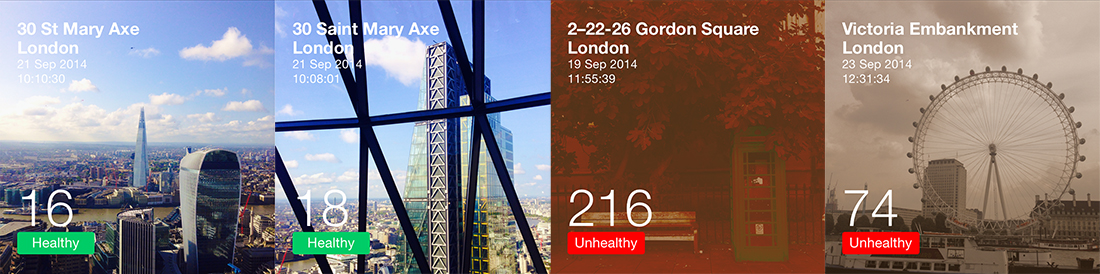
\includegraphics[scale=.4]{images/instaNO2.jpg}
\end{adjustbox}
  \caption[InstaNO2 project: photo-based visualisations]{InstaNO2: photo-based visualisations \cite{Lin2014}.}
  \label{fig:photo_based_instaNO2}
\end{figure}

\subsection{Tangible approaches}
Other approaches have made use of tangible objects to visualise air pollution in a more engaging way. The Human Sensor project \cite{InvisibleDust2016} employs wearable art and in-city performances to reveal changes in pollution levels. Similarly, WearAir, \cite{Kim2010} is an expressive T-shirt that senses VOCs and expresses the readings making use of embedded lights. Kuznetsov et al. \cite{Kuznetsov2011} developed glowing balloons with air quality sensors for users to explore urban air quality. The \textit{IBM THINK} exhibit \cite{IBM2012} is a 123-foot long digital wall display located in New York city which renders art patterns and real time streaming visualisations  that show air quality data as well as traffic flow, energy, and water usage. This immersive in-city experience is for users to explore and understand the role of data in the world. Tangible approaches are useful because they evoke curiosity and surprise while gaining an insight of what is happening. In contrast, they are not intended for personal day to day usage but as a way of expression and art and to trigger social change. 

\begin{figure}[H]
\begin{adjustbox}{width=.8\textwidth,center=\textwidth}
  \centering
  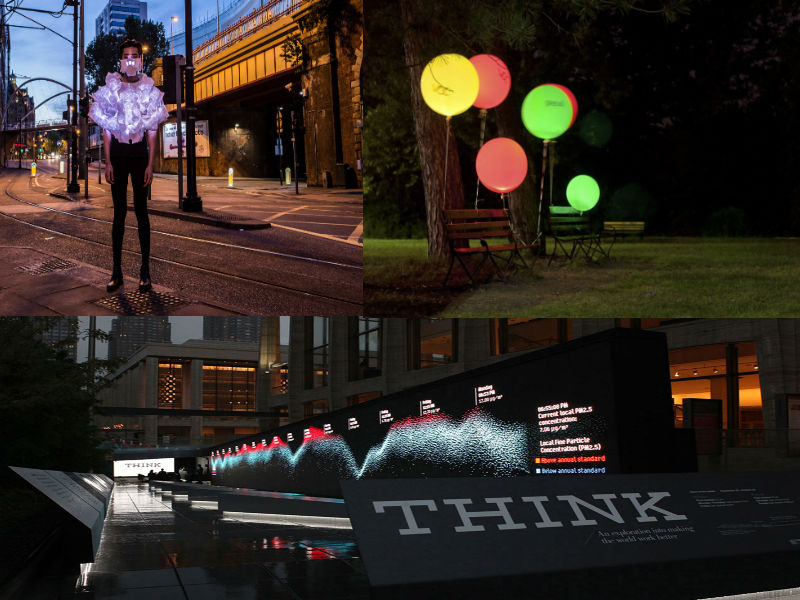
\includegraphics[scale=.4]{images/think_human_sensor_balloons.jpg}
\end{adjustbox}
  \caption[Tangible visualisations]{The human-sensor on the top-left \cite{InvisibleDust2016}, glowing balloons on the top-right \cite{Kuznetsov2011}, and IBM think on the bottom \cite{IBM2012}.}
  \label{fig:photo_based_instaNO2}
\end{figure}

